%%%%%%%%%%%%%%%%%%%%%%%%%%%%%%%%%%%%%%%%%%%%%%%%%%%%%%%%%%%%%%%%%
% Tese de Doutorado / Dept Fisica, CFM, UFSC                    %
% Andre@UFSC - 2014                                             %
%%%%%%%%%%%%%%%%%%%%%%%%%%%%%%%%%%%%%%%%%%%%%%%%%%%%%%%%%%%%%%%%%

%:::::::::::::::::::::::::::::::::::::::::::::::::::::::::::::::%
%                                                               %
%                          Capítulo 1                           %
%                                                               %
%:::::::::::::::::::::::::::::::::::::::::::::::::::::::::::::::%

%***************************************************************%
%                                                               %
%                         Introdução                            %
%                                                               %
%***************************************************************%

\chapter{Introdução}
\label{sec:intro}

%***************************************************************%
%                                                               %
%                         Intro - IFS                           %
%                                                               %
%***************************************************************%

\section{Espectroscopia de campo integral}

Na última década presenciamos uma proliferação de {\em surveys} de imageamento e
espectroscopia. {\em Surveys} como o SDSS \citep{York2000}, ALHAMBRA
\citep{Moles2008} e COSMOS \citep{Scoville2007}, para citar alguns exemplos,
permitem explorar a distribuição espectral de energia (SED\footnote{\em Spectral
Energy Distribution.}) de centenas de milhares a milhões de galáxias.
Entretanto, da forma como estes {\em surveys} são executados, há sempre um
compromisso entre a resolução espacial e a espectral. As imagens obtidas pelo
SDSS têm um boa resolução espacial, mas mapeiam a SED de forma grosseira, com
apenas $5$ filtros de banda larga ($ugriz$). Já os espectros obtidos pelo mesmo
{\em survey} possuem uma excelente resolução e cobertura espectral, mas apenas
sobre a superfície integrada da região central das galáxias.

% FIXME: Rogério - da região central das galáxias e com tamanho fixo no céu.

O melhor dos dois mundos pode ser alcançado com instrumentos que fazem
espectroscopia de campo integral (IFS\footnote{\em Integral Field
Spectroscopy.}). Instrumentos que realizam este tipo de espectroscopia consistem
em geral de um amontoado de fibras óticas, as quais alimentam um espectrógrafo
comum. Assim, depois de um processo relativamente complicado de redução de
dados, obtêm-se espectros espacialmente resolvidos com uma boa resolução
espectral e espacial. O {\em survey} CALIFA ({\em Calar Alto Legacy Integral
Field Area survey\footnote{\url{http://www.caha.es/CALIFA/}}}) está utilizando o
instrumento PMAS/PPAK do observatório Calar Alto para obter IFS de $600$
galáxias \citep{Sanchez2012}. Destas, $100$ foram disponibilizadas no primeiro
{\em Data Release} \citep[DR1]{Husemann2013}, e $200$ no segundo
\citep{GarciaBenito2015}, afirmando o caráter de legado deste {\em survey}.

Quando completado, o CALIFA terá obtido da ordem de $10^6$ espectros, quase o
mesmo que o SDSS. Porém, este não será apenas mais um {\em survey}
espectroscópico. A riqueza do CALIFA está nas informações espacialmente
resolvidas, em uma amostra representativa do universo local ($0.005 < z < 0.03$,
limitada em diâmetro angular) cobrindo a distribuição de galáxias no diagrama
cor--magnitude da nuvem azul à sequência vermelha, amostrando galáxias de todos
os tipos morfológicos (espirais, elípticas, irregulares e até mesmo alguns
sistemas em interação).

\begin{figure}
	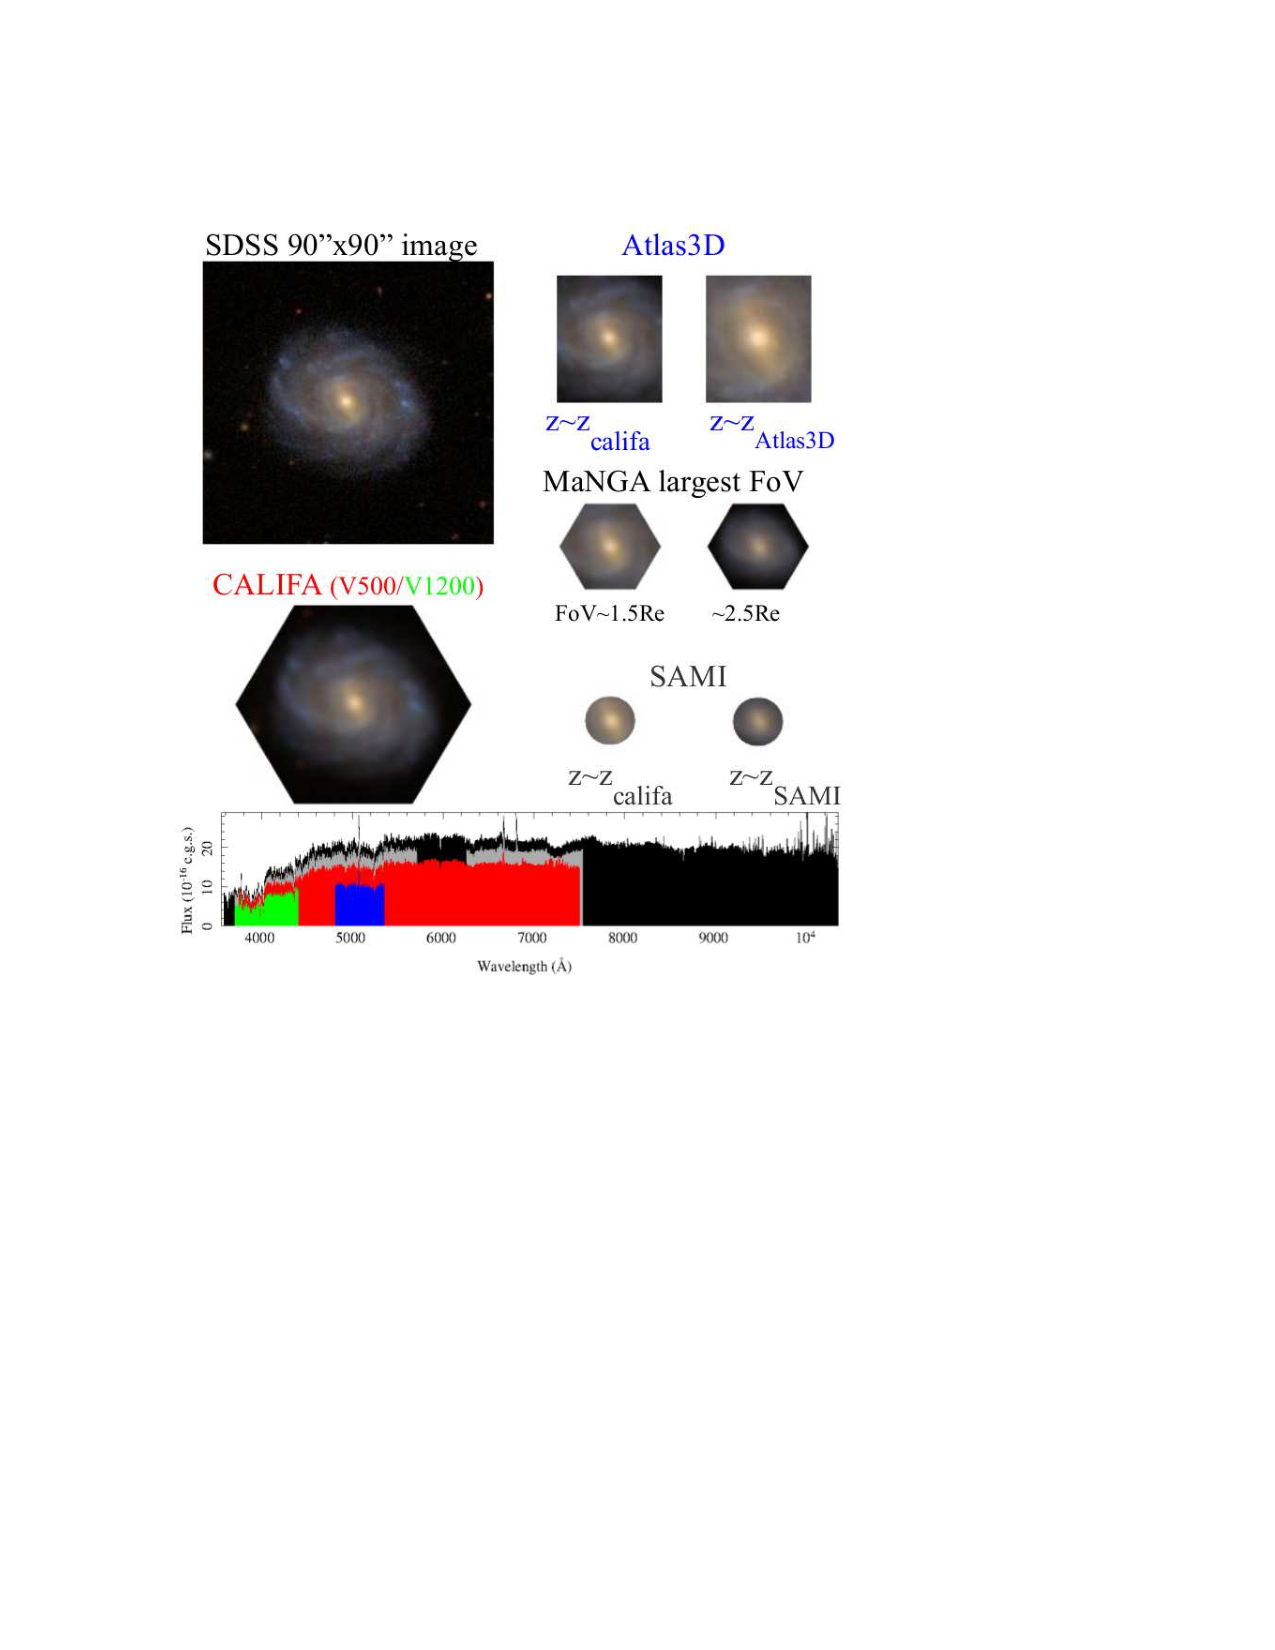
\includegraphics{figuras/surveysIFS}
	\caption[Comparação entre {\em surveys} espectroscópicos de campo integral]
	{Comparação entre {\em surveys} espectroscópicos de campo integral em execução
	atualmente. A figura superior à esquerda mostra um recorte de $90 \times
	90\,\arcs$ de NGC 5947, extraída do SDSS. Ao redor, como esta galáxia seria
	observada pelos {\em surveys} ATLAS3D, MaNGA, SAMI e CALIFA a diferentes {\em
	redshifts} típicos de cada amostra. Abaixo a faixa de comprimento de onda
	coberta por cada {\em survey} (CALIFA em verde e vermelho, ATLAS3D em azul,
	SAMI em cinza, MaNGA em preto). Retirado de \citet{Sanchez2014}.}
	\label{fig:surveysIFS}
\end{figure}

Comparado a outros {\em surveys} já realizados, como o Altas3D
\citep{Cappellari2011} ou o {\em Disk Mass Survey} (DMS) \citep{Bershady2010}, o
CALIFA cobre uma faixa muito maior de tipos morfológicos e massas. Outros {\em
surveys} que estão em andamento são o SAMI \citep{Croom2012, Bryant2015} e o
MaNGA \citep{Bundy2015}. Estes também buscam obter uma amostra grande de
galáxias, bem maior do que a do CALIFA. Entretanto, a vantagem do CALIFA está na
cobertura e amostragem espacial, observando uma maior porção de cada galáxia com
mais riqueza de detalhes. A Figura \ref{fig:surveysIFS}, mostra uma comparação
simplificada do tamanho do campo e cobertura espectral destes {\em surveys}. A
primeira Seção \ref{sec:ifs:califa} apresenta o {\em survey} CALIFA em mais
detalhes.

% FIXME: Rogério - Tabela mostrando as propriedades de cada survey seria de
% grande valia.

%***************************************************************%
%                                                               %
%                Intro - Stellar synthesis of IFS               %
%                                                               %
%***************************************************************%

\section{Síntese de população estelar espacialmente resolvida}
\label{sec:Intro:Sintese}

% FIXME: Rogério - Sugiro expandir esta seção para umas 2 ou 3 páginas. Está
% sucinto demais.

Espectros espacialmente resolvidos podem ser descritos como um cubo de dados,
com as duas primeiras dimensões sendo a posição $x$ e $y$ (ascensão reta e
declinação) e a terceira sendo o comprimento de onda. Nestes cubos, planos com
comprimento de onda constante são imagens, enquanto colunas definidas por um par
$(x, y)$ constante são espectros. Podem-se tratar estes espectros
individualmente, embora na verdade nos cubos do CALIFA os {\em
spaxels}\footnote{A palavra {\em spaxel} é uma mistura de {\em space} e {\em
pixel}, se referindo ao espectro proveniente da região espacial representada por
um {\em pixel}.} vizinhos estejam correlacionados devido ao {\em seeing} do céu
e ao processo de observação e redução. Há a queda na relação sinal/ruído (S/N)
nas regiões mais afastadas do núcleo da galáxia, onde o brilho superficial é
muito menor.
Algumas galáxias possuem outros objetos ``intrometidos'' que precisam ser
mascarados. Linhas telúricas\footnote{Linhas de absorção causadas pela
atmosfera.} também precisam ser mascaradas. Assim, em geral, é necessário um
preprocessamento visando manter um S/N mínimo e garantir um espectro livre de
contaminação. Os detalhes sobre o preprocessamento utilizado neste trabalho
estão descritos na seção 3 do Apêndice \ref{apendice:PaperResolving1}.

% FIXME: Rogério - Falar de trabalhos prévios (NIR) e das vantagens de fazer IFU
% no quesito stellar populations.

Um aspecto importante do preprocessamento utilizado é que o cubo de dados é
dividido em zonas de Voronoi, onde regiões com baixo S/N são combinadas,
formando efetivamente ``{\em spaxels} maiores''. Desta forma, o cubo original é
transformado numa matriz de zonas e comprimento de onda, onde fatias de zona
constante são espectros. Com isso, os espectros, e as máscaras e erros que os
acompanham, estão prontos para serem usados pelo próximo passo.

% FIXME: Rogério - Adicionar uma seção para explicar o starlight.

A síntese de população estelar consiste em obter a história de formação estelar
(SFH\footnote{\em Star Formation History.}) de uma galáxia utilizando modelos de
população estelar simples (SSP\footnote{\em Simple Stellar Population.}).
Ajusta-se o espectro de uma galáxia como a soma de espectros de SSPs com idades
e composições químicas distintas (levando em conta a atenuação por poeira e a
cinemática).
O resultado é um vetor de frações de luz e massa destas SSPs, que podem ser
facilmente convertidos a uma SFH conforme a prescrição de \cite{Asari2007}.
O programa utilizado é o \starlight, desenvolvido por \cite{CidFernandes2005}.

Como apresentado na Seção \ref{sec:ifs:qbick}, todos os espectros das zonas foram
passados pelo \starlight, obtendo-se o resultado da síntese como um arquivo de
saída separado para cada zona. Entretanto, para visualizar ou mesmo tentar
entender estes resultados, é preciso organizar e converter estes arquivos para
um formato mais adequado.

% FIXME: Rogério - Estas zonas são os ``pixels'' da tesselação de voronoi?
% deixar mais claro.


%***************************************************************%
%                                                               %
%                        Intro - PyCASSO                        %
%                                                               %
%***************************************************************%

\section{O nascimento do PyCASSO}

Dada a grande quantidade de dados espalhados em diversos formatos, a análise dos
resultados da síntese de populações estelares para uma determinada galáxia pode
se tornar um grande e complexo quebra-cabeças computacional. Trabalhar com todas
as galáxias do {\em survey} fica virtualmente impossível desta forma. Assim, da
necessidade de manipular os resultados da síntese dos cubos de dados das
galáxias do CALIFA, nasceu o software PyCASSO.

PyCASSO ({\em Python CALIFA \starlight Synthesis Organizer}) é um software
desenvolvido em Python com o objetivo de organizar e gerenciar os dados
produzidos pelo \starlight com base nos dados do CALIFA. O {\em survey} CALIFA é
apresentado no Capítulo \ref{sec:ifs}, que também discute os softwares QBICK e
\starlight, ferramentas básicas em nossa análise de cubos de dados. O Capítulo
\ref{sec:pycasso} apresenta a documentação do PyCASSO, e em seguida discute
alguns dos artigos publicados que o utilizam intensivamente.


%***************************************************************%
%                                                               %
%                      Intro - Decomposicao                     %
%                                                               %
%***************************************************************%

\section{Decomposição morfológica de galáxias}

Utilizando PyCASSO para trabalhar com cubos do CALIFA, buscou-se um problema
onde se pudesse utilizar a natureza multidimensional dos dados. Com o \starlight
se obtêm informações sobre a história das populações estelares, ou seja,
transforma-se comprimento de onda em tempo e luminosidade em massa. Porém, isto
é feito de forma individual, para cada {\em spaxel}. Adicionando uma análise na
distribuição de brilho da galáxia, pode-se tentar decompor o seu espectro em
componentes morfológicas, e em seguida estudar a história das populações
estelares de cada componente.

O processo de fazer a decomposição morfológica em cubos de dados espectrais de
galáxias, tal que se toma imagens de fatias em comprimento de onda
($\lambda$-a-$\lambda$), é chamado neste trabalho de decomposição morfológica
espectral. Dele resulta um conjunto de modelos morfológicos, que podem ser
manejados de forma a obter cubos de dados espectrais das componentes
morfológicas. O modelo morfológico de interesse aqui consiste em um bojo e um
disco. O Capitulo \ref{sec:morph} apresenta um breve histórico de morfologia.

A decomposição morfológica depende de uma boa caracterização da PSF ({\em Point
Spread Function}). Como parte deste trabalho, a PSF do CALIFA foi determinada
(Capítulo \ref{sec:psf}), com os resultados sendo aproveitados pela colaboração
do CALIFA, e publicados em \citet{GarciaBenito2015}. Foram feitos testes do
algoritmo de decomposição, descritos no Capítulo \ref{sec:test}, utilizando uma
galáxia sintética. Estes testes não foram exaustivos, eles apenas indicam que a
decomposição pode funcionar. Os testes incluem populações estelares compostas,
variáveis com a posição no modelo. Outro teste importante, apresentado no mesmo
capítulo, foi o efeito de usar uma PSF mal dimensionada na decomposição, com
largura diferente da PSF do cubo de dados.

O Capítulo \ref{sec:Decomp} descreve em detalhes o algoritmo de decomposição
morfológica espectral. O preprocessamento dos dados inclui (mas não se limita a)
regularizar a cinemática da galáxia, combinar espectros em imagens, calcular
erros correlacionados. O ajuste das imagens ao modelo bojo--disco é feito
utilizando o programa IMFIT \citep{Erwin2015}, descrito na seção
\ref{sec:morph:comp:ajuste}. Foi escolhida uma amostra de galáxias que
potencialmente podem ser decompostas em bojos e discos, resultando num conjunto
de cubos espectrais de componentes bojo e disco de cada galáxia desta amostra.
Os cubos destas componentes são tratados exatamente da mesma forma que uma
galáxia ao serem passados pelo \starlight. Utilizando PyCASSO, os resultados da
síntese espectral foram analisados e comparados com a síntese da galáxia
original.

% FIXME: Rogério - Sugestões:
%
% * Fazer uma revisão sobre estudos de pop. estelares e morfologia em galáxias.
% * Contextualizar qual o ganho de fazer isso em 3d.
% * Já tem algum resultado de síntese ou análise de morfologia em 3d publicado?
% Qual a diferença entre estes e o que tu  propões aqui?
% * Qual a dificuldade de manipular os dados de IFU em um survey?
% * Qual o objetivo do teu trabalho? Qual é o passo científico que a tua tese
% vai dar?
% 
% Em resumo, faltou deixar claro qual o problema!

% End of this chapter
